\documentclass[border=4pt]{standalone}

\usepackage{amsmath}
\usepackage{tikz}
\usepackage{mathdots}
\usepackage{yhmath}
\usepackage{cancel}
\usepackage{color}
\usepackage{siunitx}
\usepackage{array}
\usepackage{multirow}
\usepackage{amssymb}
\usepackage{gensymb}
\usepackage{tabularx}
\usepackage{booktabs}
\usetikzlibrary{fadings}
\usetikzlibrary{patterns}


\begin{document}
 


\tikzset{every picture/.style={line width=0.75pt}} %set default line width to 0.75pt        

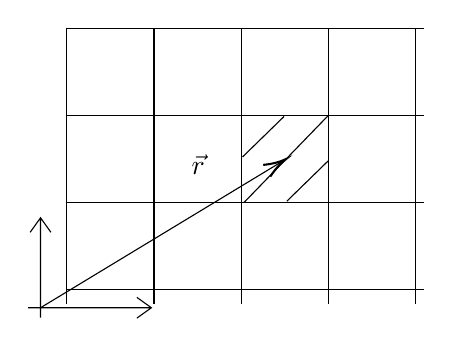
\begin{tikzpicture}[x=0.75pt,y=0.75pt,yscale=-1,xscale=1]
%uncomment if require: \path (0,300); %set diagram left start at 0, and has height of 300

%Shape: Grid [id:dp2756243967663181] 
\draw  [draw opacity=0] (100,116) -- (272,116) -- (272,249) -- (100,249) -- cycle ; \draw   (100,116) -- (100,249)(142,116) -- (142,249)(184,116) -- (184,249)(226,116) -- (226,249)(268,116) -- (268,249) ; \draw   (100,116) -- (272,116)(100,158) -- (272,158)(100,200) -- (272,200)(100,242) -- (272,242) ; \draw    ;
%Straight Lines [id:da4102072462587749] 
\draw    (87.33,250.67) -- (203.96,180.04) ;
\draw [shift={(205.67,179)}, rotate = 508.8] [color={rgb, 255:red, 0; green, 0; blue, 0 }  ][line width=0.75]    (10.93,-3.29) .. controls (6.95,-1.4) and (3.31,-0.3) .. (0,0) .. controls (3.31,0.3) and (6.95,1.4) .. (10.93,3.29)   ;

%Shape: Axis 2D [id:dp7678505414359664] 
\draw  (81.4,250.67) -- (140.73,250.67)(87.33,207.32) -- (87.33,255.48) (133.73,245.67) -- (140.73,250.67) -- (133.73,255.67) (82.33,214.32) -- (87.33,207.32) -- (92.33,214.32)  ;
%Straight Lines [id:da4739568879416445] 
\draw    (184.67,178) -- (204.67,158.5) ;


%Straight Lines [id:da42691499757265117] 
\draw    (206,199.33) -- (226,179.83) ;


%Straight Lines [id:da12812814796506133] 
\draw    (185.33,200) -- (226,158) ;



% Text Node
\draw (163.33,181.67) node    {$\vec{r}$};


\end{tikzpicture}
\end{document}
